\documentclass[12pt]{article}
\usepackage{authblk}
\usepackage{amsmath}
\usepackage{amssymb}
\usepackage{graphicx}
\usepackage{caption}

\captionsetup{font=scriptsize}
\title{\textbf{Prediction of Remaining Useful Life (RUL) of Batteries using Neural ODE based GRU}}
\author{Shubham Mate}

\author{Nandanavanam VS Sai Saketh}


\affil{Department of Mathematical Sciences, IIT (BHU), Varanasi}
\affil{\texttt{mate.shubhamvijay.mat23@itbhu.ac.in, nvssai.saketh.mat23@itbhu.ac.in}}

\date{November 2024}

\begin{document}
	
	\maketitle
	\section{Objective}
		
		\footnotesize{To predict the Remaining Useful Life (RUL) of a battery by giving 20 observations which consists of the various features of the batteries using a neural ODE without using the capacity (mAH) feature which is used in traditional methods. The model was to be trained on the given dataset.}
		\subsection{Dataset}
			\footnotesize{The dataset to be used is the Battery Remaining Useful Life Prediction dataset on Kaggle. The Hawaii Natural Energy Institute examined 14 NMC-LCO 18650 batteries with a nominal capacity of 2.8 Ah, which were cycled over 1000 times at 25°C with a CC-CV charge rate of C/2 rate and discharge rate of 1.5C. This data released by Hawaii Natural Energy Institute was used to make this dataset. It contains the following features:
			\begin{description}
				\item[Cycle Index] The Cycle number of current cycle
				\item[Discharge Time (s)] time that takes the voltage to reach its minimum value in one discharge cycle.
				\item[Decrement 3.6-3.4V (s)] It represents the time taken for voltage to drop from 3.6V to 3.4V during a discharge cycle.
				\item[Max. Voltage Dischar. (V)] The initial and maximum voltage in the discharging phase.
				\item[Min. Voltage Charg. (V)] The initial value of voltage when charging.
				\item[Time at 4.15V (s)] The time to reach 4.15V in charging phase.
				\item[Time constant current (s)] The time in which the current stays constant at its max. value.
				\item[Charging time (s)] The total time for charging.
				\item[RUL] The Remaining Useful Life of battery after every cycle.
			\end{description}}
	\section{Mathematical Formulation}
		\footnotesize{In this section, we'll look at and recap the mathematical formulation of the various techniques and components used in the model}
		\subsection{Neural ODE}
			\footnotesize{Numerous Models build complicated transformations by composing a sequence of
			transformations to the input or a maintained hidden state. These transformations are mathematically expressed as:
			\begin{equation*}
				\mathbf{z}_{t+1} = \mathbf{z}_{t} + f(\mathbf{z}_{t}, \theta_{t})
			\end{equation*}
			where $t \in \{0, \dots, T \}$ and $h_{t} \in \mathbb{R}$. These iterative
			updates can be seen as an Euler discretization of a continuous transformation. Neural ODE aims to parameterize the continuous dynamics of $z_{t}$ given by the equation:
			\begin{equation*}
				\frac{d\mathbf{z}(t)}{dt} = f(\mathbf{z}(t), t, \theta) 
			\end{equation*}
			The output of Neural ODE is generated with a black box differential equation solver. Therefore, the $\mathbf{z}(T)$ can be obtained by:
			\begin{equation*}
				\mathbf{z}(T) = \mathbf{z}(t_0) + \int_{t_{0}}^T \mathbf{f}(\mathbf{z}(t), t; \mathbf{\theta}) \, dt = \text{ODESolve}(\mathbf{z}(t_0), f, t_0, T, \theta)
			\end{equation*}
			In order to avoid backpropogating through the black box differential solver, Neural ODE uses adjoint sensitivity method to calculate required gradients. At every point, it maintains an adjoint state $\mathbf{a}(t)$ whose dynamics are given by another ODE:
			\begin{equation*}
				\frac{d\mathbf{a}(t)}{dt} = -\mathbf{a}(t)^T \frac{\partial \mathbf{f}(\mathbf{z}(t), t; \mathbf{\theta})}{\partial \mathbf{z}(t)}
			\end{equation*}
			Another ODE solver is used to solve the dynamics of $\mathbf{a}(t)$.
			The Gradient $\frac{d\mathbf{L}}{d\theta}$ is finally computed by the equation:
			\begin{equation*}
				\frac{d\mathcal{L}}{d\mathbf{\theta}} = \int_0^T \mathbf{a}(t)^T \frac{\partial \mathbf{f}(\mathbf{z}(t), t; \mathbf{\theta})}{\partial \mathbf{\theta}} dt
			\end{equation*}
			We use Neural ODEs to model the dynamics of the hidden state of a GRU.}
		\subsection{Neural ODE based GRU}
			\footnotesize{RNN (Recurrent Neural Network) is a type of neural network which maintains a hidden state $\mathbf{h}_t$ which gets updated each time a new input is fed into it. This allows it to remember information from previous inputs. This makes them suitable to model sequential/time-series data in which current input may be dependant on previous inputs.
			\\
			GRU (Gated Recurrent Unit) is a variation of RNNs where each unit has an update gate ($z_t$) and reset gate ($r_t$) which allows them to select what information should be maintained by hidden states and what information should be forgotten. The equations for the GRU are:
			\begin{equation}
				z_t = \sigma(\mathbf{W}_z \mathbf{x}_t + \mathbf{U}_z \mathbf{h}_{t-1} + \mathbf{b}_z)
			\end{equation}
			\begin{equation}
				r_t = \sigma(\mathbf{W}_r \mathbf{x}_t + \mathbf{U}_r \mathbf{h}_{t-1} + \mathbf{b}_r)
			\end{equation}
			\begin{equation}
				\tilde{\mathbf{h}}_t = \tanh(\mathbf{W}_h \mathbf{x}_t + \mathbf{U}_h (r_t \odot \mathbf{h}_{t-1}) + \mathbf{b}_h)
			\end{equation}
			\begin{equation}
				\mathbf{h}_t = (1 - z_t) \odot \mathbf{h}_{t-1} + z_t \odot \tilde{\mathbf{h}}_t
			\end{equation}
			To incorporate a Neural ODE to update the hidden state, we give the following method:
			\\
			Suppose we have two inputs $\mathbf{x}_{t_1}$ and $\mathbf{x}_{t_2}$. Let us define a function UpdateGRU($\mathbf{x}$, $\mathbf{h}_t$) which takes an input and current hidden state and updates the states according to the equations given above. We also define a function $f$ (a neural network) with parameters $\theta$
			\\
			We use the following method to get the output:
			\begin{equation*}
				\mathbf{h}_{t_1} = \mathbf{UpdateGRU}(\mathbf{x}_{t_1}, \mathbf{h}_{t_0})
			\end{equation*}
			\begin{equation*}
				\mathbf{h}_{t_1} = \mathbf{ODESolve}(\mathbf{h}_{t_1}, f, t_1, t_2, \theta)
			\end{equation*}
			\begin{equation*}
				\mathbf{h}_{t_2} = \mathbf{UpdateGRU}(\mathbf{x}_{t_2}, \mathbf{h}_{t_1})
			\end{equation*}
			This helps us model the continuous dynamics of the hidden state of GRU in between the updates, which can help us even model time series data with irregular time interval.}
	\newpage
	\section{Methodology}
	\footnotesize{In this section, we'll look at various methods performed on the data to make the model.}
		\subsection{Feature Creation}
			\begin{figure}[h]
				\centering
				\begin{minipage}{0.45\textwidth}
					\centering
					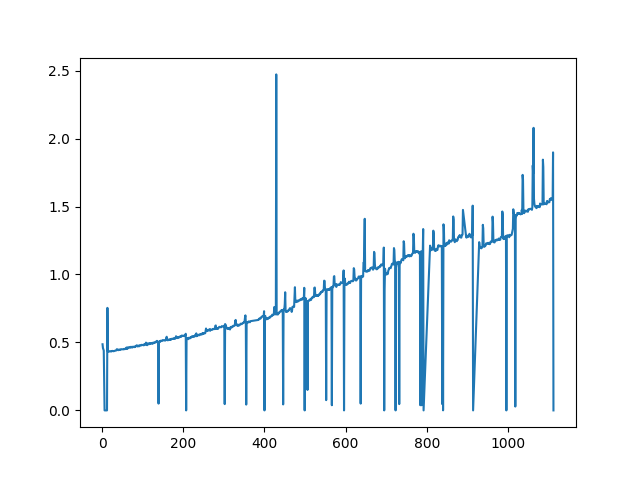
\includegraphics[width=\textwidth]{imgs/LogChargeToTimeConstCurrentPlt.png}
					\caption{Plot of log(Charging time (s) / Time Constant Current (s)) vs Cycle Index}
					\label{fig:plot1}
				\end{minipage}
				\hfill
				\begin{minipage}{0.45\textwidth}
					\centering
					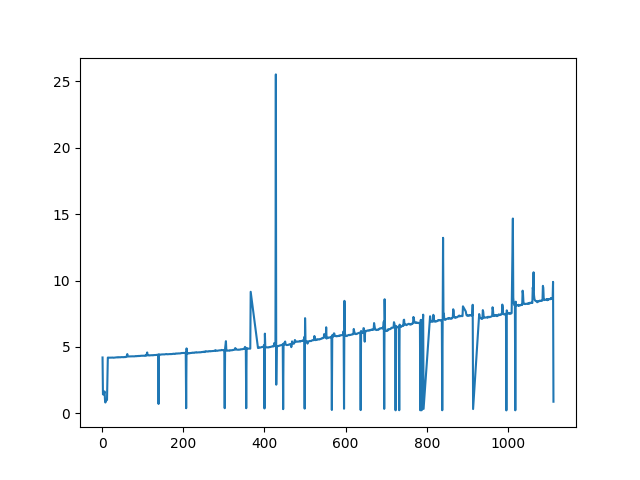
\includegraphics[width=\textwidth]{imgs/ChargeToDischargePlt.png}
					\caption{Plot of Charging time (s) / Discharge Time (s) vs Cycle Index}
					\label{fig:plot2}
				\end{minipage}
			\end{figure}
			\footnotesize{Through trial and error, we found that the ratio of Charging time to Discharging time along with the log of ratio of Charging Time to Time Constant Current showed decent correlation with the Cycle Index. Thus, we added this to our features.}
		\subsection{Smoothing}
			\begin{figure}[h]
				\centering
				\begin{minipage}{0.32\textwidth}
					\centering
					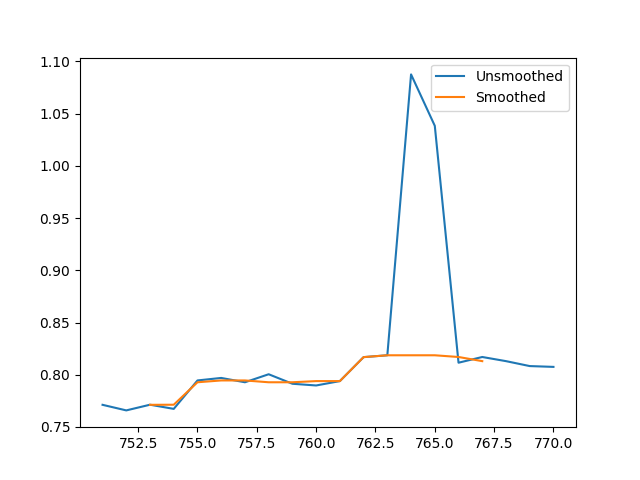
\includegraphics[width=\textwidth]{imgs/smoothing_1.png}
				\end{minipage}
				\hfill
				\begin{minipage}{0.32\textwidth}
					\centering
					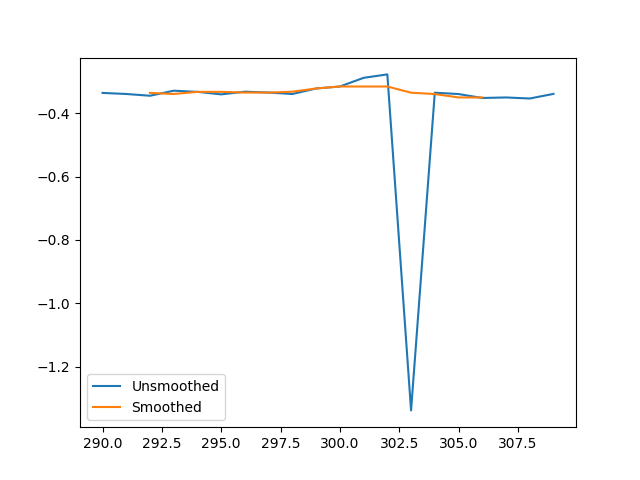
\includegraphics[width=\textwidth]{imgs/smoothing_2.png}
				\end{minipage}
				\hfill
				\begin{minipage}{0.32\textwidth}
					\centering
					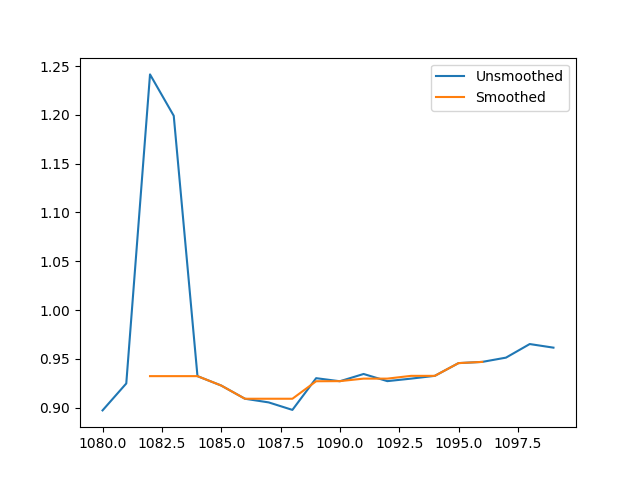
\includegraphics[width=\textwidth]{imgs/smoothing_3.png}
				\end{minipage}
				\caption{Effect of Median Smoothing on features within the sliding window}
				\label{fig:three_plots}
			\end{figure}
			\footnotesize{There are many spikes within the dataset due to noise. This can affect our model's performance. So, we employed smoothing technique to remove this noise. We used Median Smoothing with a kernel size of 5 to smooth out the data within a sliding window.}
		\subsection{Training and Evaluation}
		The dataset contains measurement of 14 different batteries. Out of these, 10 batteries were used as training data and rest 4 were used as testing data. We used a Robust Scaler for scaling the features, as this scaler is robust to outliers which are present in the data due to noise. The RUL is standardised in the usual way i.e $z = \frac{\mathbf{x} - \mu}{\sigma}$
		\\
		We used a sliding window approach with size of the window set as 20 such that each data point will be $D_i = \{(x_{i-20}, \dots, x_i), (t_{i-20}, \dots, t_i), y_i\}$ where $(x_{i-20}, \dots, x_i)$ was supplied to the GRU and $(t_{i-20}, \dots, t_i)$ was used by Neural ODE to model the dynamics of the hidden state. Previously mentioned Median Smoothing is applied to each datapoint and then the data is converted into batches with Dataset and Dataloader provided by PyTorch. We also used L2 Regularization to prevent overfitting.
		\\
		\footnotesize{We used a Mean Squared Error (MSE) as the loss function for our training and Root Mean Square Error (RMSE) along with other metrics as the evaluation metric.}
		Our method achieved an average RMSE of \textbf{52.606754} on the test dataset.
		
		\begin{table}[h]
		\centering
		\begin{tabular}{|c|c|c|c|c|}
			\hline
			Model & RMSE & MSE & MAE & R2 Score \\
			\hline
			Proposed Model & 52.606 & 2787.640 & 44.349 &  0.9722 \\
			\hline
		\end{tabular}
		\caption{Results of Evaluation on training set}
		\label{tab:simple_table}
		\end{table}
		
		\begin{figure}[h]
			\centering
			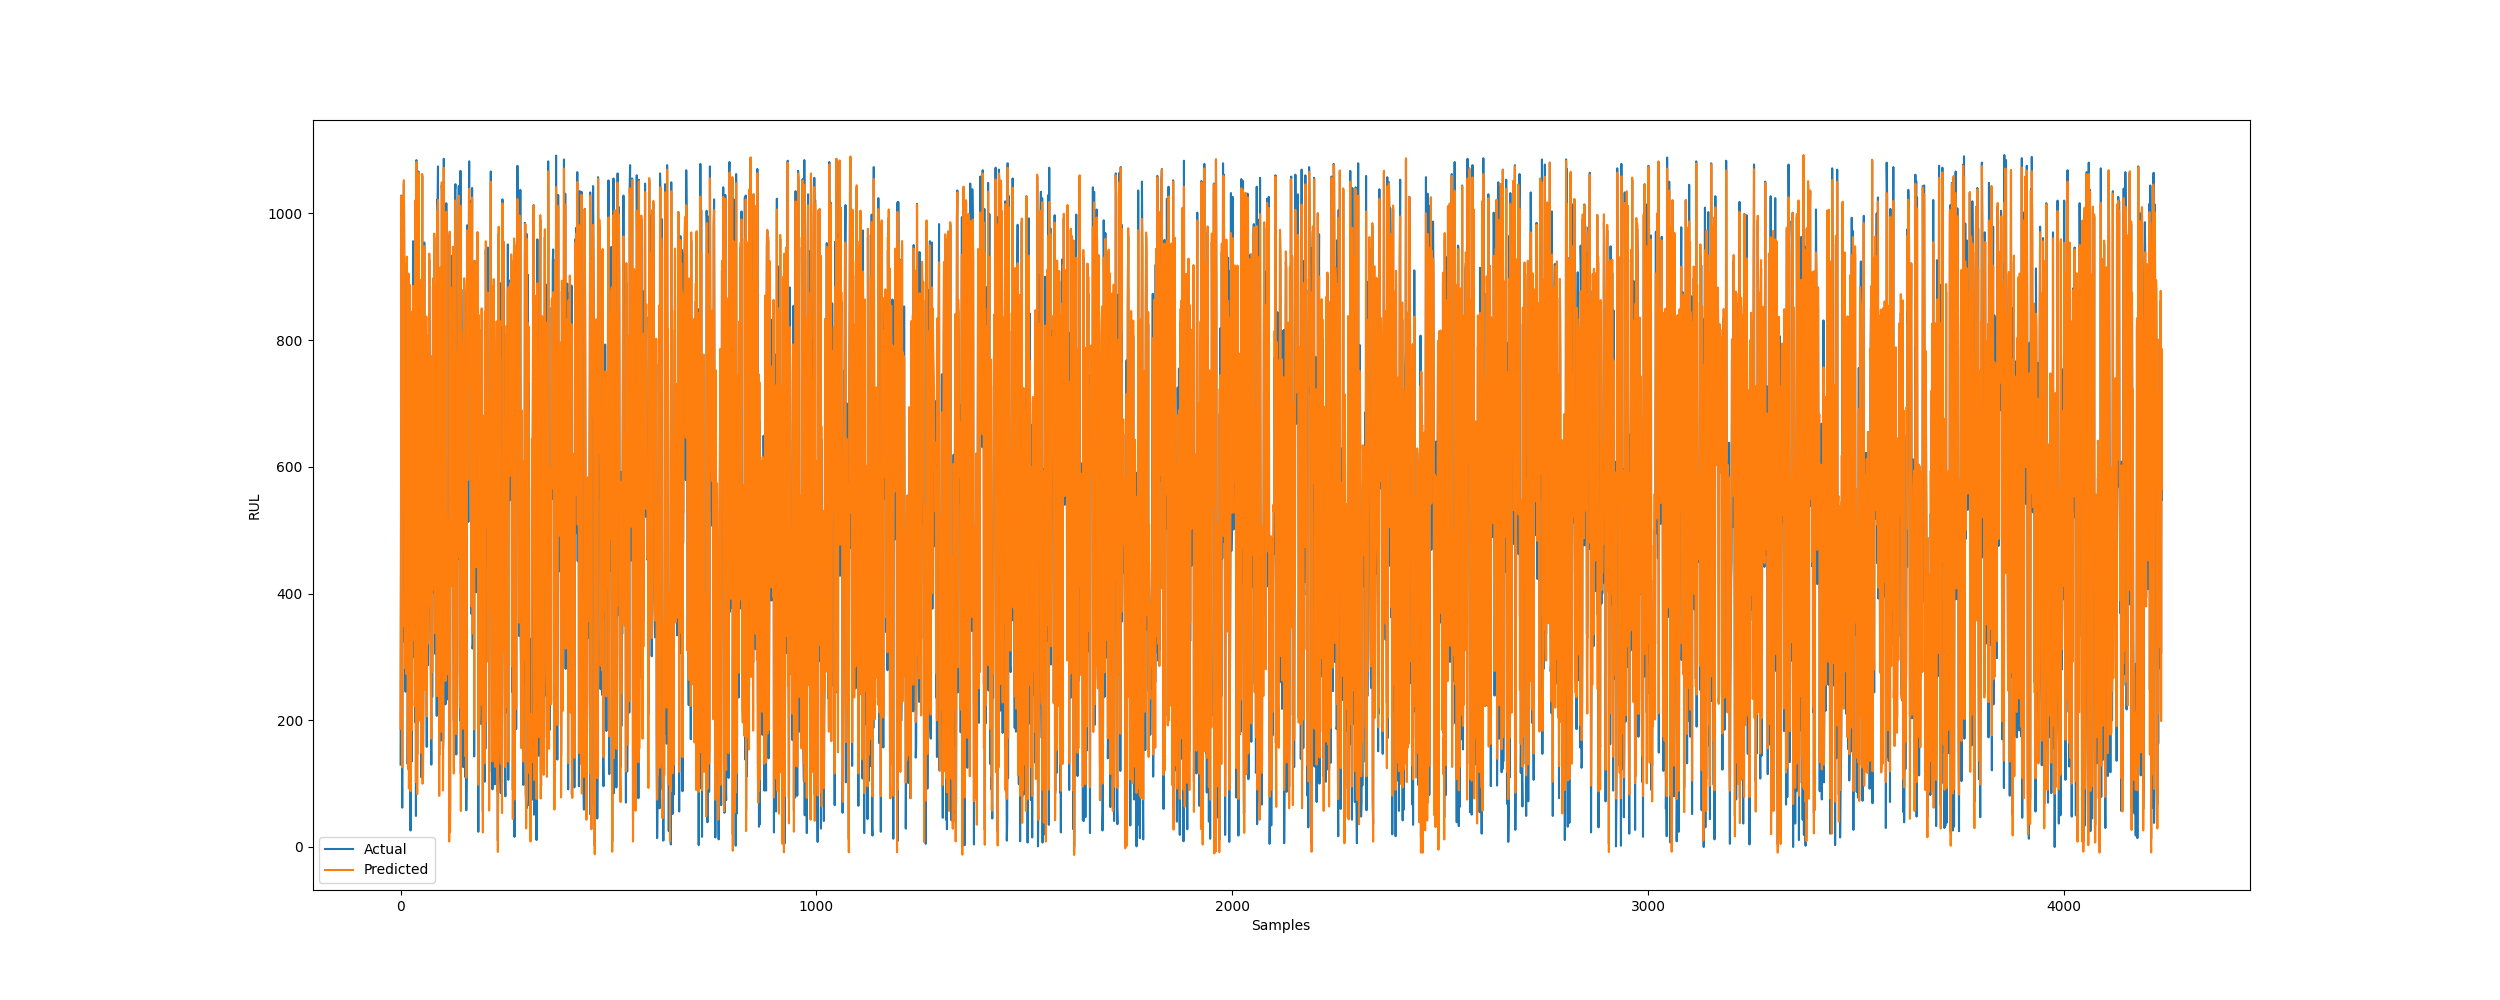
\includegraphics[width=\textwidth]{imgs/predicted.png}
			\caption{Predicted RUL and Actual RUL}
		\end{figure}
		\newpage
	\section{\large{Novelty and Advantages over previous methods}}
	\begin{table}[h]
		\centering
		\begin{tabular}{|c|c|}
			\hline
			Model & RMSE \\
			\hline
			PSR-SVR & 191.83 \\
			\hline
			GRU-RNN & 127.65 \\
			\hline
			CNN-LSTM & 176.63 \\
			\hline
			\textbf{Proposed Model} & \textbf{52.606} \\
			\hline
		\end{tabular}
		\caption{Comparison with other methods}
		\label{tab:comparison}
	\end{table}
	Neural ODE based GRU presents a novel approach over traditional methods in discrete time involving RNNs, GRUs and LSTMs by leveraging continuous time dynamics. Some advantages of this approach are:
	\begin{itemize}
		\item \textbf{Flexibility with Irregularly Sampled Data:} Since Neural ODEs naturally support irregular time intervals, Neural ODE-based GRU models can effectively handle missing or irregularly spaced data points. This dataset has some data missing for certain cycle indices, which can be effectively modelled by this method
		
		\item \textbf{Reduced Memory Footprint and Efficient Backpropagation:} Neural ODEs use a memory-efficient adjoint sensitivity method for backpropagation, requiring only the initial and final states for gradient calculations. This drastically reduces the memory consumption during training and makes the model more scalable to larger datasets and longer sequences.
		
		\item \textbf{Improved Long-Term Dependency Capture:} By modeling the hidden state evolution as a continuous process, Neural ODE-based GRU can effectively capture long-term dependencies and avoid issues like vanishing gradients commonly found in traditional recurrent neural networks, which improves performance in tasks with long-range temporal dependencies.
		
		\item \textbf{Robust to overfitting:} Also, from our observation, modelling of the continuous time dynamics of hidden state prevents overfitting and can also act as a regularization technique.
	\end{itemize}
	These advantages makes this model suitable for this task.
\end{document}